Para realizar este ejercicio, debemos de tener en cuenta que el tamaño máximo de la frontera será de $2$ por el valor dado
\begin{center}
    \begin{tabular}{|c|c|c|c|}
        \hline
        Estado actual & Frontera (cola de prioridad) y costo acumulado & Podado & Camino \\
        \hline
        $s_0$ & $[s_2:2]$ & - & $[s_0]$ \\
        \hline
        $s_2$ & $[s_4:4], [s_1:6]$ & - & $[s_0,s_2]$ \\
        \hline
        $s_4$ & $[s_1:6], [s_3:7],$ & $[s_4:11]$ & $[s_0,s_2,s_4]$ \\
        \hline
        $s_1$ & $[s_3:7],$ & -  & $[s_0,s_2,s_4, s_1]$ \\
        \hline
        $s_3$ & - & -  & $[s_0,s_2,s_4, s_1, s_3]$ \\
        \hline
    \end{tabular}
\end{center}

Podemos ver lo que sucede en el siguiente arbol

\begin{center} 
    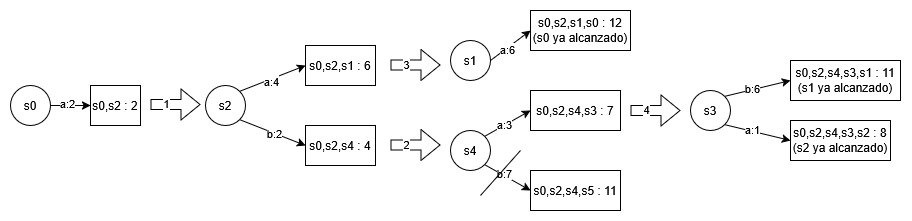
\includegraphics[height = 4cm]{respuestas/img/treeE8.png}
\end{center}

Notemos que con una cola de prioridad no es posible llegar al estado final con este valor de $k$ con lo que se generaron $5$ caminos pero ninguno fue exitoso.\\

